
\providecommand{\myrootdir}{..}
\documentclass[\myrootdir/main.tex]{subfiles}

\begin{document}

\chapter{Information Extraction Techniques}
\label{sec:models}
%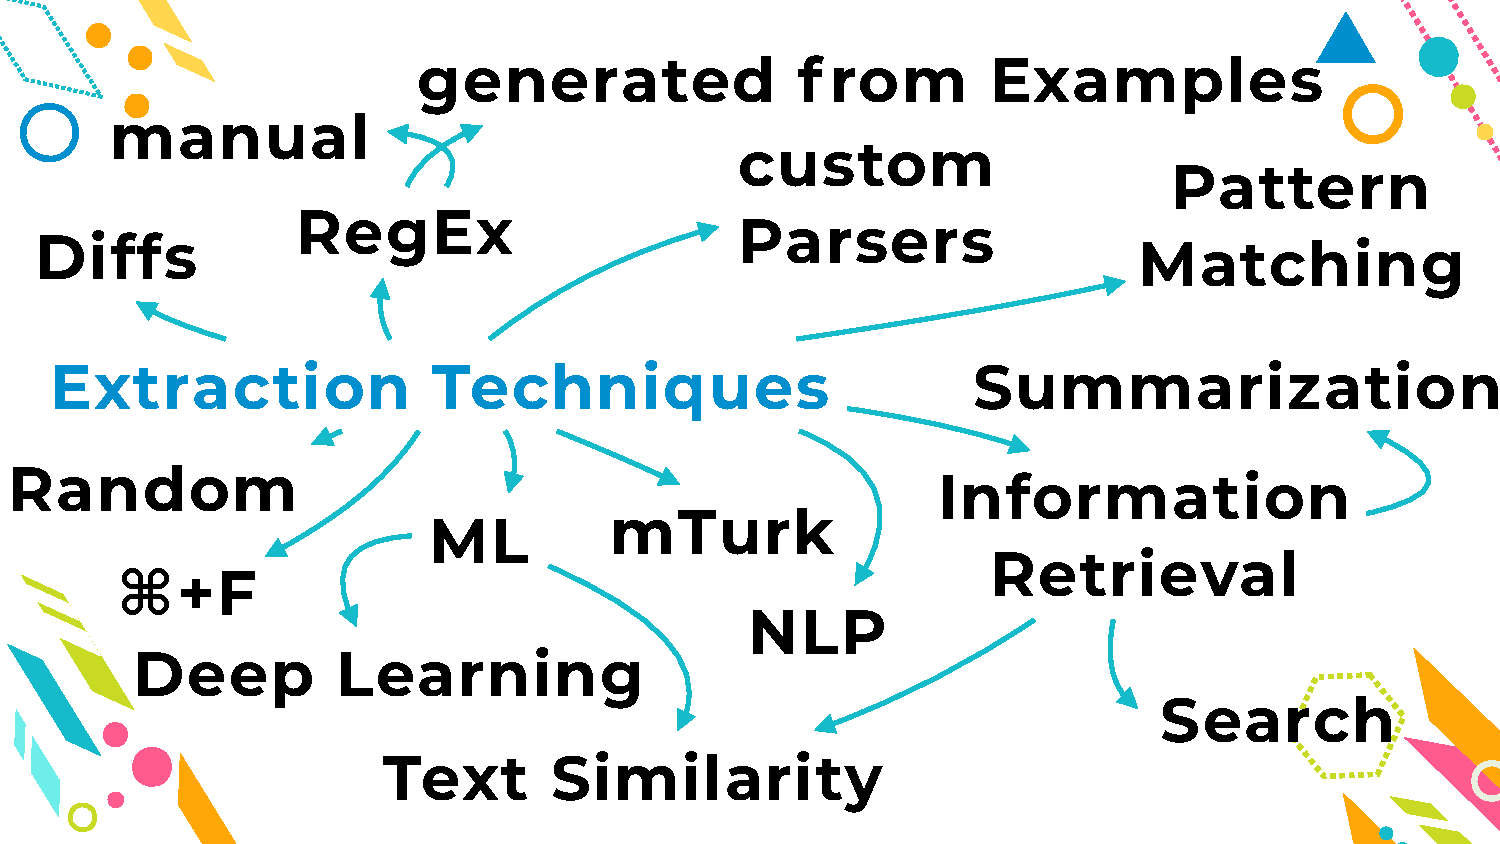
\includegraphics[page=1, width=\textwidth, trim={0.5cm 0.5cm 0.5cm 0.5cm}, clip]{img/RetreatSeptemberSlides.pdf}
Many different information extraction techniques ... this section describes the conceptional / theoretical results of our thesis ...
We create a model to characterize BLIE techniques so we can discuss their similarities and differences more clearly.
Additionally we present a complimentary model for IE tasks, to describe use cases for BLIE techniques in a structured way.
From our analysis of build logs we share our notion of the extractable information within a build log.

\section{Characteristics of a Build Log}
The idea of CI is, to integrate new software changes fast and often to catch errors early. After making a change, the developer commits and pushes it to a shared source code repository. Companies often use a specific CI server, e.g. Travis CI, linked to their source code repository. A CI build might then be triggered by a push on specific branches or after a pull request was created. When such a CI build is triggered, it typically runs through these stages:
\begin{itemize}
	\item Pulling in the new, changed version of the source code.
	\item Running static analysis tools~\cite{zampetti2017open}.
	\item Building the software, i.e. compiling and packaging it~\cite{phillips2014understanding}.
	\item Running automated tests.
\end{itemize}
However these are only \emph{typical} stages and there is a high variability in the CI build processes of different software projects \mention{citation needed, zampetti2017open?}. Some smaller projects might just use CI to make sure their code compiles as a minimal check before reviewing a pull request, other projects might have various stages of extensive automated testing.

Independent from the actual composition of the CI build process, most software tools used within a build will write out log messages to the console \mention{citation needed, paper about usages of console.log?}. Often, the console output is the only means to for a build tool to communicate with its users. Tools print progress updates, error and warning messages on the console.

The structure of this output is chosen by every tool themselves. Many have implicit or explicit structuring rules, some adhere to predefined standards \mention{phpunit, ruby, xuint output?}. However, when anlayzing build logs we might not have access to the exact build configuration (which tools are used in which order) or might not have access to a useable definition of the output sturcture of a specific tool. Therefore we describe build logs as semi-structured.

Semi-structured for build logs means for us that the log text is:
\begin{itemize}
	\item[implicitly stuructured], we do not have access to explicit structuring elements or an explicit structure description
	\item[irregular], the structure changes without notice \todo{we saw this in our data collection, random newlines}
\end{itemize}

\plan{a build consists of various steps, executed by different tools, these are often orchestrated by at least one overarching tool. // picture: overarching tool travis and it calls different tools which tehn output sequentiall, travis sometimes outputs something in between -> that is how the build log is made up // we have this structure though it is not always apparent from the build log / edges between the systems can look very different, mostly no agreed model, we: look at differen techniques to extract certain pieces of information \emph{without complete parsing the whole log in to a structure} -> we don't necesarrily want to understand the whole log sturcture just extract one specifi information relevant to us}

\subsection{Comparison to Runtime Logs}
\todo{or did we do that in related work enough?}

\section{Our Model for Extractable Information in Build Logs}
\begin{figure}[h]
  \centering
\includegraphics[page=2, width=\textwidth, trim={0.5cm 0.5cm 0.5cm 0.5cm}, clip]{img/flow-of-research.pdf}
  \caption{Information extractable from build logs}
  \label{fig:build-log-information-draft}
\end{figure}
Continuous integration build logs contain a huge amount of information about the various stages in the CI build they correspond to. In this section we present our model to more precisely describe our notion of a information extractable from a CI build log.

A \emph{build log information} for us has:
\begin{itemize}
	\item a \emph{textual representation} within the build log, more specifically a substring of the log string
\end{itemize}
With this build information items can be hierachically ordered by their textual representations containing each other.

\begin{figure}[h]
	\centering
	\includegraphics[width=\textwidth]{img/mt-graphics-BuildLogInformation.pdf}
	\caption{Build Log Information}
	\label{fig:build-log-information}
\end{figure}
During our inital exploration \& data collection for the \emph{Failing Build Log Data Set}, wanted to get an impression about the information one would want to extract from a build log. Within the Travis CI build logs we found various different informations possibly interesting to be extracted
\begin{itemize}
	\item[Travis Build Step] A Travis CI build consists of several build steps defined within the Travis CI configuration language. Within the build log each of these steps are framed by \lstinline{travis_fold:start:<build step name>} and \lstinline{travis_fold:end:<build step name>}.
	      A build step contains
	      \begin{itemize}
		      \item[Build Step Name] The string Travis uses to identify the step within start \& end statements.
		      \item[Build Step Output] The output generated during the build step. The textual representation of the \texttt{Build Step Output} is the substring between the start \& end statements.
	      \end{itemize}
	\item[Travis Timing] Travis can measure the time of specified sections of the build process. It represents those by \lstinline{travis_time:start:<timing section id>} and \lstinline{travis_time:end:<timing section id>:start=<start time>,finish=<finish time>,duration=<duration>}
\end{itemize}

\todo{differentiate Travis CI specific things, explain high variability for instantiations}
\todo{give at least one concrete example instantiation, best from a log in the data set, not too long so maybe it goes in the abstract?, picture/graphic with marked parts here?}


\section{Our Model for Information Extraction Techniques}
\begin{figure}[h]
	\centering
	\includegraphics[page=3, width=\textwidth, trim={0.5cm 0.5cm 0.5cm 0.5cm}, clip]{img/flow-of-research.pdf}
	\caption{Model for an information extraction technique}
	\label{fig:model-ie-technique}
\end{figure}
\plan{model = making a picture with boxes to visualize what we are talking about}
A build log information extraction technique (BLIE technique) consumes a build log (text file) and produces a certain output (text). \todo{make picture, output can be contained in log or not, can be continuous substring or selected lines etc.}.
\begin{itemize}
	\item{Target}{Extractable Information} each extraction technique \todo{instantiation!} targets a specific information
	\item{Setup Overhead}{Time}
	\item{Performance}{Performance} split into learning performance
	\item \textbf{Configuration Scope} for one repository/project, a language/logkind, global
\end{itemize}

Example instantiations of this task later in this chapter, namely for the three techniques we are comparing: PROSE program synthesis, IR text similarity, and simple keyword search. \todo{ref?}

\section{Our Model for Information Extraction Tasks}
\begin{figure}[h]
	\centering
	\includegraphics[page=4, width=\textwidth, trim={0.5cm 0.5cm 0.5cm 0.5cm}, clip]{img/flow-of-research.pdf}
	\caption{Model for information extraction task}
	\label{fig:modelt-ie-task}
\end{figure}
aims to describe an information extraction task of a developer or a researcher.
\begin{itemize}
	\item \todo{describe all classes}
	\item{Setup Overhead}{Time}
	\item{Performance}{Performance} split into learning performance
\end{itemize}
\todo{give 2-3 concrete example instantiations here}


\section{PROSE Program Synthesis}
\begin{figure}[h]
  \centering
\includegraphics[page=2, width=\textwidth, trim={0.5cm 0.5cm 0.5cm 0.5cm}, clip]{img/RetreatSeptemberSlides.pdf}
  \caption{Synthesizing regular expression programs by example using PROSE}
  \label{fig:prose-explanation}
\end{figure}
\todo{explanation of process, the way our tool does it, instantiate model of extraction technique, probably no additional theoretical stuff really needed here?, describe regex programs}

\section{Text Similarity}
\begin{figure}[h]
  \centering
\includegraphics[page=3, width=\textwidth, trim={0.5cm 0.5cm 0.5cm 0.5cm}, clip]{img/RetreatSeptemberSlides.pdf}
  \caption{Extracting information using text similarity}
  \label{fig:text-similarity-explanation}
\end{figure}
\todo{explanation of process, the way our tool does it, instantiate model of extraction technique, probably no additional theoretical stuff really needed here?}

\section{Keyword search}
\begin{figure}[h]
  \centering
\includegraphics[page=4, width=\textwidth, trim={0.5cm 0.5cm 0.5cm 0.5cm}, clip]{img/RetreatSeptemberSlides.pdf}
  \caption{Extracting information using keyword search}
  \label{fig:keword-search-explanation}
\end{figure}
\todo{explanation of process, the way our tool does it, instantiate model of extraction technique, probably no additional theoretical stuff really needed here?}

\section{Further Techniques}
\todo{maybe: instantiate model, or at least partly talk about it}
\todo{diffing, manual regex?, other summarization?, BART? <- we could reference that from related work then}

\end{document}
